\documentclass[11pt,a4paper]{article}

% ─── Packages ───────────────────────────────────────────────────────────────
\usepackage[margin=1in]{geometry}
\usepackage{graphicx} % for \includegraphics of the two architecture diagrams (PNG)
\usepackage{amsmath,amssymb,amsthm}
\usepackage{booktabs}
\usepackage{array}
\usepackage{tabularx}
\usepackage{longtable}
\usepackage{hyperref}
\usepackage{xcolor}
\usepackage{enumitem}
\usepackage{microtype}
\usepackage{fancyhdr}
\usepackage{titlesec}
\usepackage{tcolorbox}
\usepackage{listings}
\usepackage{caption}
\usepackage{cite}
\usepackage{setspace}
\usepackage{parskip}
\usepackage[T1]{fontenc}
\usepackage{lmodern}
\usepackage{cleveref} % for \cref cross-references (sections, tables); no figures this revision
\usepackage[section]{placeins} % force every floating table to resolve before the next \section,
  % so a backlog of [htbp] tables can never drift past the bibliography
\tcbuselibrary{skins,breakable,theorems}

\newenvironment{property}[1][]
{
  \begin{tcolorbox}[
    title={#1},
    colback=white,
    colframe=black!50,
    fonttitle=\bfseries
  ]
}
{
  \end{tcolorbox}
}

% ─── Color Definitions ──────────────────────────────────────────────────────
\definecolor{navyblue}{RGB}{27,42,74}
\definecolor{slateblue}{RGB}{74,127,191}
\definecolor{lightgray}{RGB}{247,249,252}
\definecolor{warningred}{RGB}{139,26,26}
\definecolor{warningyellow}{RGB}{204,122,0}

% ─── Hyperref Setup ─────────────────────────────────────────────────────────
\hypersetup{
  colorlinks=true,
  linkcolor=navyblue,
  citecolor=slateblue,
  urlcolor=slateblue,
  pdftitle={Autonomous Signals: A New Ontology for AI Agents},
  pdfauthor={Bc77},
  pdfkeywords={autonomous agents, signal models, AI safety, containment,
               kill switch, agentic AI, LLM safety, ButterClaw}
}

% ─── Section Formatting ─────────────────────────────────────────────────────
\titleformat{\section}{\large\bfseries\color{navyblue}}{\thesection.}{0.8em}{}[\color{navyblue}\titlerule]
\titleformat{\subsection}{\normalsize\bfseries\color{navyblue}}{\thesubsection}{0.8em}{}
\titleformat{\subsubsection}{\normalsize\bfseries\color{slateblue}}{\thesubsubsection}{0.8em}{}

% ─── Callout Boxes ──────────────────────────────────────────────────────────
\newtcolorbox{definitionbox}[1][]{enhanced,breakable,colback=blue!5!white,
  colframe=slateblue,fonttitle=\small\bfseries\color{white},title={Definition},
  left=6pt,right=6pt,top=4pt,bottom=4pt,#1}
\newtcolorbox{warningbox}[1][]{enhanced,breakable,colback=red!5!white,
  colframe=warningred,fonttitle=\small\bfseries\color{warningred},
  title={Critical Failure Mode},left=6pt,right=6pt,top=4pt,bottom=4pt,#1}
\newtcolorbox{importantbox}[1][]{enhanced,breakable,colback=yellow!8!white,
  colframe=warningyellow,fonttitle=\small\bfseries\color{warningyellow},
  title={Core Claim},left=6pt,right=6pt,top=4pt,bottom=4pt,#1}
\newtcolorbox{pullquotebox}{enhanced,breakable,colback=white,colframe=slateblue,
  toprule=1.5pt,bottomrule=1.5pt,leftrule=0pt,rightrule=0pt,
  fontupper=\itshape\color{navyblue},left=12pt,right=12pt,top=8pt,bottom=8pt}

% ─── Listings ───────────────────────────────────────────────────────────────
\lstset{basicstyle=\small\ttfamily\color{navyblue},backgroundcolor=\color{lightgray},
  frame=single,framerule=0.4pt,rulecolor=\color{slateblue},xleftmargin=8pt,
  xrightmargin=8pt,breaklines=true,keepspaces=true,columns=fullflexible}
\newcolumntype{L}[1]{>{\raggedright\arraybackslash}p{#1}}

% ─── Page Style ─────────────────────────────────────────────────────────────
\pagestyle{fancy}
\fancyhf{}
\fancyhead[L]{\small\color{navyblue}\textit{Autonomous Signals: A New Ontology for AI Agents}}
\fancyhead[R]{\small\color{navyblue}Bc77}
\fancyfoot[C]{\small\thepage}
\renewcommand{\headrulewidth}{0.4pt}
\setlength{\parskip}{4pt}
\setlength{\parindent}{0pt}

% ════════════════════════════════════════════════════════════════════════════
\begin{document}
% ════════════════════════════════════════════════════════════════════════════

\begin{center}
  {\LARGE\bfseries\color{navyblue}
    Autonomous Signals: A New Ontology for AI Agents}

  \vspace{8pt}
  {\large\color{slateblue}\itshape
    The ButterClaw Containment Architecture and the Conceptual Shift\\
    from Language Models to Signal Models}

  \vspace{6pt}
  {\normalsize Bc77}

  \vspace{3pt}
  {\footnotesize ButterClaw Tech}

  \vspace{1pt}
  {\footnotesize ORCID 0009-0001-2162-1397}

  \vspace{2pt}
  {\small\color{gray} research@butterclaw.tech \quad\textbullet\quad October 2026}
\end{center}

\vspace{4pt}\noindent\rule{\linewidth}{1.5pt}\vspace{2pt}

\begin{abstract}
\noindent
The field of artificial intelligence has long operated under a vocabulary inherited from its
earliest paradigms: ``language models,'' ``chatbots,'' ``agents,'' ``assistants.'' This paper
argues that these terms are not merely imprecise---they are \emph{epistemically dangerous}.
When the ontological frame does not match a system's actual behavior, safety guarantees built on
that frame become structurally unsound.

We propose a principled reframing: large language models are more accurately described as
\emph{signal models}---systems that transduce, transform, and emit structured semantic
signals---and autonomous AI agents are more precisely understood as \emph{autonomous signal
loops}, self-routing information processes that accumulate context, initiate actions, and resolve
without continuous human mediation. This reframing surfaces a new safety surface defined by
signal boundaries, loop depth, side-effect potential, and termination conditions rather than
token probabilities and prompt structures.

To address this surface, we introduce \textbf{ButterClaw}---a containment-first reference
architecture for safe autonomous signal deployment, now at implementation version
\textbf{v0.9.2}. ButterClaw defines six architectural layers, a five-hemisphere reasoning model
that separates decisive, skeptical, speculative, self-improving, and fleet-level cognition into
independently scheduled LLM passes, a named policy evaluation runtime (DRIFT) spanning three
signal-lifecycle scopes, a three-tier kill switch model (Signal Pause, Loop Drain, Hard
Termination) with a concrete credential-destruction mechanism (Gibson), four containment
primitives (Boundary, Depth, Consent, Observability) mapped onto the runtime's enforced
invariants, and a formal threat model for adversarial signal injection.
\end{abstract}

\vspace{2em}
\hrule
\vspace{1em}
\noindent \footnotesize \textit{\textbf{Licensing:} The ButterClaw runtime architecture and source code are licensed under Apache-2.0. This whitepaper is licensed under a Creative Commons Attribution 4.0 International License (CC-BY-4.0).}

\noindent\rule{\linewidth}{0.6pt}\vspace{4pt}

\noindent\textbf{Keywords:} autonomous signals, signal models, agentic AI, AI safety,
containment architecture, kill switch, signal loops, ButterClaw\\
\textbf{Primary Classification:} cs.AI \quad\textbf{Cross-list:} cs.SE, cs.SY

\noindent\rule{\linewidth}{0.6pt}\vspace{4pt}

\tableofcontents\newpage

% ────────────────────────────────────────────────────────────────────────────
\section{Introduction: The Naming Problem in AI}
% ────────────────────────────────────────────────────────────────────────────

Language is infrastructure. The terms a technical community uses to describe its artifacts
do not merely label---they constrain. They determine which properties get measured, which failure
modes get anticipated, and which safety primitives get designed. The field of artificial
intelligence has accumulated a vocabulary increasingly mismatched with the systems it seeks to
describe. This mismatch is not a cosmetic inconvenience. It is a structural risk.

The canonical AI vocabulary---``language model,'' ``chatbot,'' ``assistant,'' ``agent''---was
assembled when these systems were narrow, stateless, and principally text-bound. Contemporary
frontier models can initiate tool calls, traverse multi-step reasoning chains, maintain context
across thousands of turns, spawn subagents, write and execute code, modify files, dispatch
emails, and transact with external APIs---all within a single inference episode. Yet we still
call them ``language models'' and frame their safety properties in terms of content policy and
output filtering.

\begin{importantbox}
Imprecise ontology produces imprecise safety guarantees. The names we give AI systems determine
the failure modes we protect against---and therefore the failure modes we leave unprotected.
\end{importantbox}

\subsection{Why Terminology Shapes Safety}

AI agents modeled as ``language models''---token-prediction engines---receive safety engineering
appropriate for text generation: output filtering, probability thresholds, toxicity classifiers.
They do not receive safety engineering appropriate for autonomous signal loops: loop depth
bounding, context membrane enforcement, federated kill switches, orphan signal detection. The
gap between what is needed and what is provided is the direct product of the nomenclature gap.

\subsection{Paper Roadmap}

This paper proposes a systematic reframing. Section~\ref{sec:signalmodels} develops the signal
model concept. Section~\ref{sec:autonomoussignals} defines autonomous signals.
Section~\ref{sec:signalloops} introduces signal loop architecture.
Section~\ref{sec:butterclaw} presents ButterClaw, including its five-hemisphere reasoning model,
its DRIFT policy engine, its memory substrate, and its fleet detection stack as implemented in
v0.9.2. Sections~\ref{sec:killswitch} and~\ref{sec:containment} address kill switch design
(including the Gibson credential-destruction mechanism) and containment modeling, mapped onto the
runtime's enforced invariants. Section~\ref{sec:relatedwork} situates ButterClaw against
conventional agent frameworks and prior kill-switch and prompt-injection research.
Section~\ref{sec:artifact} describes the released software artifact, its SDK, and how to cite
this work. Section~\ref{sec:openproblems} treats open problems. Section~\ref{sec:conclusion}
concludes.

% ────────────────────────────────────────────────────────────────────────────
\section{From Language Models to Signal Models}
\label{sec:signalmodels}
% ────────────────────────────────────────────────────────────────────────────

\subsection{What a Language Model Actually Does}

At the computational substrate level, a ``language model'' computes a probability distribution
over the next token $x_{n+1} \in \Sigma$ given an input sequence
$\mathbf{x} = (x_1, \ldots, x_n)$. This describes the \emph{mechanism}, not the
\emph{function}. The function is the transformation of an input semantic structure into an output
semantic structure with semantic payload, implicit commitments, and potential real-world
consequences.

\begin{pullquotebox}
``Token prediction is the mechanism of signal transduction, not the function of signal
transformation. Describing a large language model purely as a next-token predictor is like
describing a telephone as a membrane vibration device.''
\end{pullquotebox}

\subsection{Redefining the Unit of Analysis: The Signal}

\begin{definitionbox}[title=Definition 2.1 --- Signal]
A \textbf{signal} is a structured unit of information characterized by:
(1)~a \emph{semantic payload}---propositional content with interpretable meaning;
(2)~a \emph{temporal context}---a timestamp, session state, or causal ordering;
(3)~a \emph{transformative intent}---the change to be effected in the receiving system; and
(4)~a \emph{provenance record}---a traceable origin identifying the initiating agent or process.
\end{definitionbox}

\subsection{Framing Comparison}

\begin{table}[htbp]
  \centering\small
  \caption{Language Model Framing vs.\ Signal Model Framing}
  \label{tab:framing}
  \begin{tabularx}{\linewidth}{L{2.8cm} L{4.5cm} L{5.5cm}}
    \toprule
    \textbf{Dimension} & \textbf{Language Model} & \textbf{Signal Model} \\
    \midrule
    Primary Unit       & Token / sequence          & Signal (payload + provenance) \\
    Input Type         & Text prompt               & Structured signal with intent \& context \\
    Output Type        & Text completion           & Transformed signal w/ side-effect commitment \\
    Temporal Awareness & Implicit (context window) & Explicit (timestamp, causal ordering) \\
    Safety Surface     & Content (toxicity, accuracy) & Boundaries, loop depth, consent, observability \\
    Containment Req.   & Filtering, classifiers    & Isolation, loop bounding, kill switch, orphan detection \\
    Failure Vocabulary & Hallucination, jailbreak  & Loop divergence, orphan propagation, consent bypass \\
    \bottomrule
  \end{tabularx}
\end{table}

\subsection{Implications for Design and Evaluation}

Evaluation suites must expand to include signal-level metrics: side-effect potential per
inference call, loop initiation rate, external state modification surface, consent solicitation
frequency. Architecture decisions must treat signal isolation as a first-class design constraint.
Safety engineering must be defined at signal boundaries, depths, and consent surfaces---not at
output content alone.

% ────────────────────────────────────────────────────────────────────────────
\section{Autonomous Signals}
\label{sec:autonomoussignals}
% ────────────────────────────────────────────────────────────────────────────

\subsection{Definition}

\begin{definitionbox}[title=Definition 3.1 --- Autonomous Signal]
An \textbf{autonomous signal} is a signal that initiates, routes, and resolves itself without
requiring \emph{continuous} human mediation at each step of its lifecycle. It carries sufficient
context, routing logic, and resolution criteria to propagate through a computational environment
and effect state changes independently, subject only to the constraints of its containing
architecture.
\end{definitionbox}

\subsection{Anatomy}

An autonomous signal has five structural components:
\textbf{Origin} (provenance record, preserved throughout lifecycle);
\textbf{Payload} (semantic content);
\textbf{Routing Logic} (next-hop specification, potentially model-generated);
\textbf{Resolution Criteria} (conditions for signal closure);
\textbf{Termination Condition} (conditions for cessation regardless of resolution state).

\subsection{Properties}

\textbf{Persistence}: State maintained across multiple steps.
\textbf{Self-Routing}: Next destination determined at least partially from payload + environment.
\textbf{Context Accumulation}: Tool outputs and environmental state appended at each hop.
\textbf{Side-Effect Potential}: External state (files, APIs, communications) may be modified.

\subsection{Taxonomy}

\textbf{Reactive}: Triggered by external event; bounded single-path response.
\textbf{Proactive}: System-initiated on schedule or condition; higher autonomy.
\textbf{Recursive}: Spawns child signals; creates tree/graph propagation structures.
\textbf{Federated}: Crosses organizational or system trust boundaries.

\subsection{Signal Lifecycle Diagram}

\begin{lstlisting}[caption={Autonomous Signal Lifecycle in ButterClaw}]
[INITIATION]  Origin recorded . Payload formed . Provenance stamped
     |
[CLASSIFICATION]  Signal type . Containment tier . Consent surface
     |
[ROUTING]  Next-hop resolved . Loop depth++ . Context membrane check
     |
[CONTEXT ACCUMULATION]  Tool results appended . State captured
     |
+--[ Resolution Criteria Met? ]----------------------------------+
| YES --> [RESOLUTION] --> Audit record written . Loop closed    |
| NO  --> Return to ROUTING  (depth check enforced)             |
+----------------------------------------------------------------+
     |
[TERMINATION / ESCALATION]
  Normal     : resolution criteria satisfied
  Timeout    : termination condition triggered
  Kill       : kill switch event received
  Escalation : loop depth exceeded -> human review queue
     |
[AUDIT & REPLAY LOG WRITTEN]
\end{lstlisting}

% ────────────────────────────────────────────────────────────────────────────
\section{Signal Loops: The Architecture of Agentic Behavior}
\label{sec:signalloops}
% ────────────────────────────────────────────────────────────────────────────

\begin{definitionbox}[title=Definition 4.1 --- Signal Loop]
A \textbf{signal loop} is a closed-loop computational structure in which the output of a signal
transformation re-enters the system as input to a subsequent transformation, without requiring
external human re-initiation between cycles. Signal loops are the fundamental architectural unit
of agentic behavior.
\end{definitionbox}

\subsection{Loop Typology}

\begin{table}[htbp]
  \centering\small
  \caption{Signal Loop Typology}
  \label{tab:loops}
  \begin{tabularx}{\linewidth}{L{2.3cm} L{3.5cm} L{2cm} L{5cm}}
    \toprule
    \textbf{Type} & \textbf{Description} & \textbf{Risk} & \textbf{Containment Priority} \\
    \midrule
    Open Loop      & Unidirectional; no feedback                    & Low       & Audit logging; output validation \\
    Closed Loop    & Output re-enters as input; criterion governs exit & Medium & Depth limit; timeout; resolution validation \\
    Recursive Loop & Spawns child loops; tree/graph structure        & High      & Stack depth accounting; child inherits parent constraints \\
    Federated Loop & Hops cross trust/system boundary               & Very High & Cross-domain trust; federated kill switch; provenance attestation \\
    \bottomrule
  \end{tabularx}
\end{table}

\subsection{The Stability Problem}

For signal loops driven by large language models, the routing function is a high-dimensional
nonlinear transformation learned from data. Formal stability proofs are not currently tractable.
This makes empirical loop monitoring and depth-bounding essential safety primitives---in the
absence of provable convergence, hard limits must be enforced architecturally.

\subsection{Loop Depth Bounding}

\emph{Loop depth} is the number of autonomous signal transformations since the initiating signal
was created without human re-initiation. \emph{Maximum permitted depth} is a hard architectural
configuration parameter---the ceiling beyond which no signal may propagate regardless of routing
logic. Correct configuration is context-dependent: a code generation agent may safely operate at
depth~10; an autonomous financial transaction agent may require depth~2 with mandatory consent
gates at every level. In the reference implementation this ceiling is enforced concretely by the
\texttt{ChainExecutor}, which executes a maximum of ten steps per chain under a sixty-second total
timeout (Invariant I-07; \cref{sec:invariant-mapping}).

\subsection{Inter-Agent Signal Propagation}

In multi-agent systems, containment requires graph-level properties: total propagation path depth
must be bounded; trust attestations must be verified at each inter-agent boundary; kill switch
events must propagate bidirectionally through the graph.

% ────────────────────────────────────────────────────────────────────────────
\section{The ButterClaw Architecture}
\label{sec:butterclaw}
% ────────────────────────────────────────────────────────────────────────────

\begin{definitionbox}[title=Definition 5.1 --- ButterClaw]
\textbf{ButterClaw} is a six-layer reference architecture for autonomous signal deployment.
Its central design commitment is that containment is a first-class architectural primitive.
Every signal that enters a ButterClaw-compliant system is classified, bounded, monitored, and
subject to controlled termination from the moment of ingestion.
\end{definitionbox}

\subsection{Core Design Principles}

\begin{enumerate}[itemsep=2pt]
  \item \textbf{Signal Isolation}: Signals isolated by default; sharing requires policy authorization.
  \item \textbf{Loop Bounding}: Hard depth limit enforced architecturally, not at application layer.
  \item \textbf{Consent Surfaces}: External state modification requires verified consent traversal.
  \item \textbf{Observable State}: No ``dark'' signals; all state emitted to monitoring surface in real time.
  \item \textbf{Graceful Degradation}: Kill events preserve state, drain in-flight signals, lock forensic records.
\end{enumerate}

\subsection{Architectural Layers}

\begin{figure}[htbp]
\centering
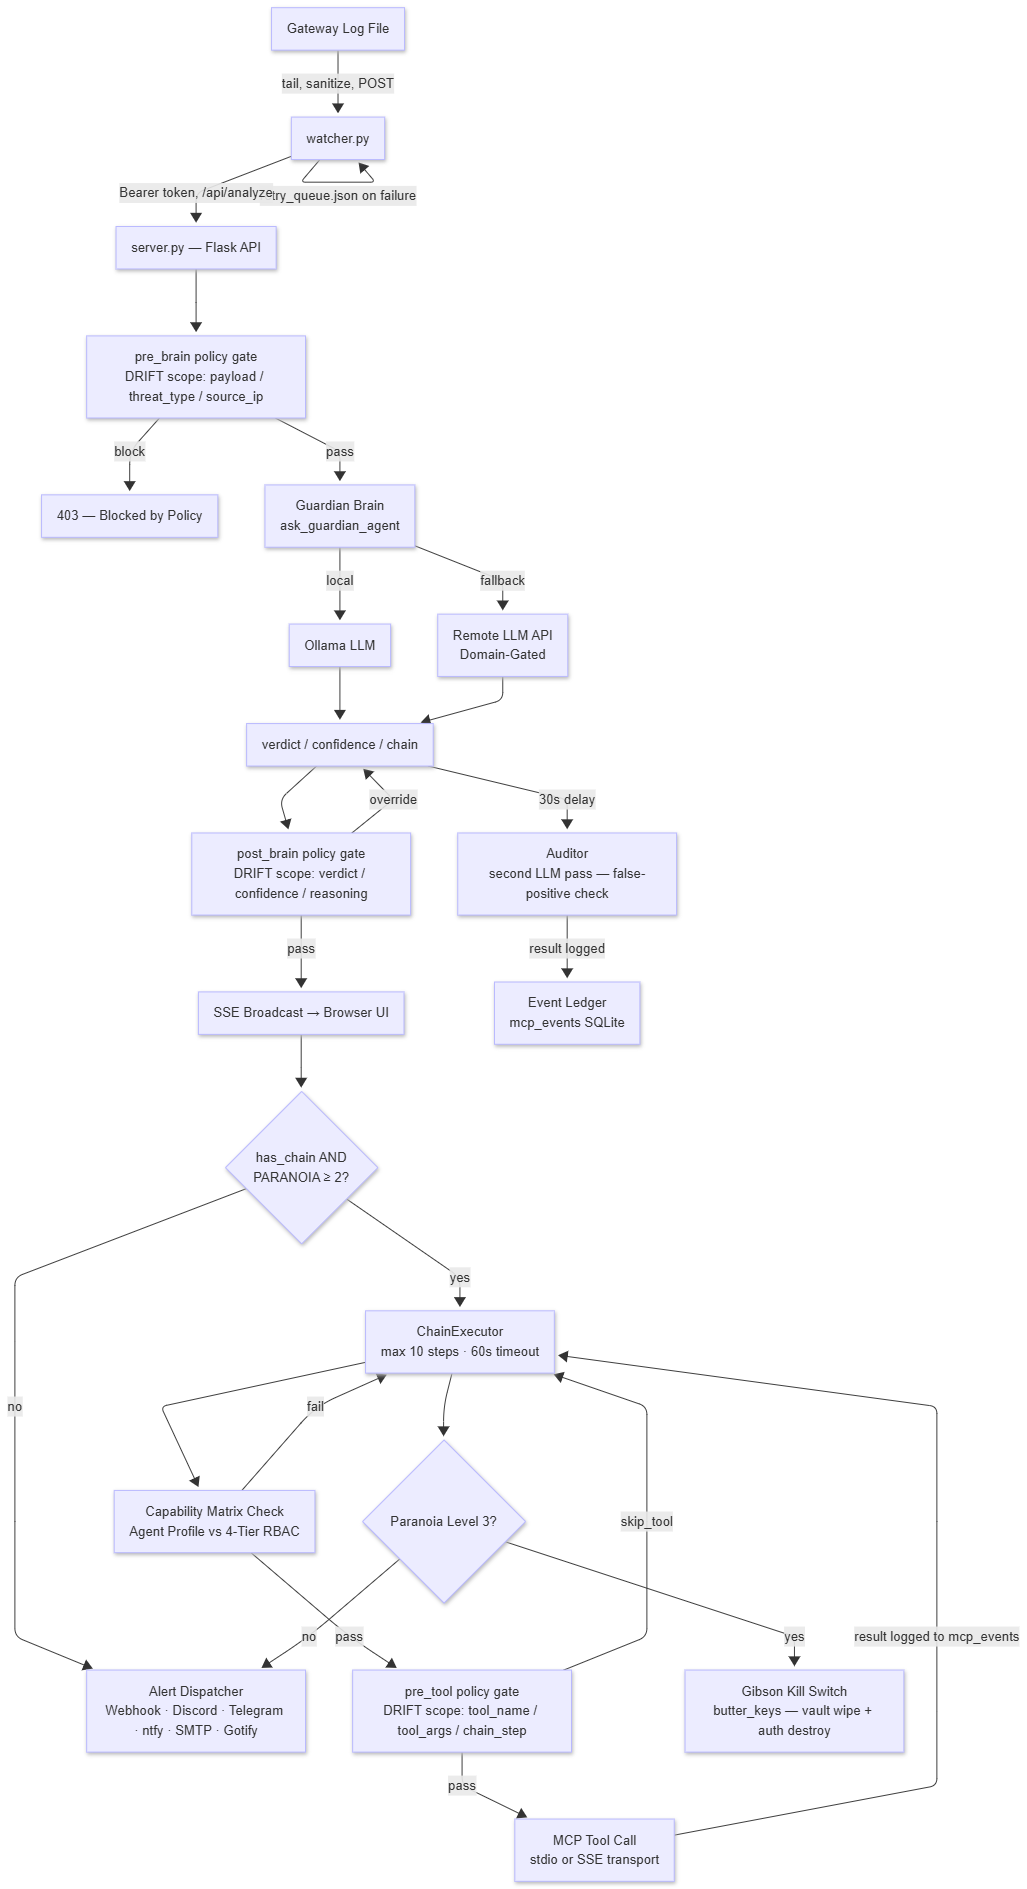
\includegraphics[width=\linewidth,height=0.75\textheight,keepaspectratio]{../diagrams/1.png}
\caption{High-level data flow through the ButterClaw runtime. Requests enter via the Watcher
Daemon (Layer~0), traverse the \texttt{pre\_brain} context membrane (Layer~1), are evaluated by
the Guardian Brain hemisphere (Layer~2), monitored by the Loop Monitor (Layer~3), executed by the
ChainExecutor/RTC (Layer~4), and written to the immutable audit log (Layer~5).}
\label{fig:highlevel}
\end{figure}

Figure~\ref{fig:highlevel} illustrates the complete data flow through all six layers.

\textbf{Layer 0 --- Signal Ingestion \& Classification}: Single ingestion endpoint; UUID stamping;
provenance; containment tier assignment. Unclassifiable signals quarantined.

\textbf{Layer 1 --- Context Membrane}: Stateful semantic boundary. Maintains signal integrity
via cryptographic payload authentication. Enforces per-signal context scoping to prevent
contamination. Primary defense against prompt injection into signal payloads.

\textbf{Layer 2 --- Routing Engine}: Policy-graph-governed dispatch. Permitted routing paths,
mandatory consent checkpoints, and dead-end rules for depth-exceeded signals. As of v0.9.0--v0.9.2
this layer's decision surface is implemented concretely by the five reasoning hemispheres
(\cref{sec:hemispheres}) and arbitrated by the DRIFT policy engine (\cref{sec:drift}).

\textbf{Layer 3 --- Loop Monitor}: Real-time registry of active loops, depths, initiation times,
and side-effect logs. Evaluates invariants at every depth increment. Issues kill commands on
threshold violations.

\textbf{Layer 4 --- Resolution \& Termination Controller (RTC)}: Processes resolution events and
termination events. Implements the three-tier kill switch. Ensures no signal continues after a
termination event for its signal tree.

\textbf{Layer 5 --- Audit \& Replay Layer}: Append-only, cryptographically chained audit log.
Full replay capability for forensic analysis. Availability is a \emph{prerequisite} for signal
execution, not an optional monitoring enhancement.

\subsection{The Context Membrane}

The context membrane operates at the semantic layer, not the network layer. Its core operation is
\emph{context scoping}: at each hop, the signal's available context is exactly the information
legitimately accumulated through its lifecycle plus any information explicitly released by
routing policy. Its secondary operation is \emph{payload authentication}: modification between
hops without authorization triggers quarantine and Loop Monitor alert. This defends against
\emph{context contamination injection}---a class of attack in which a malicious signal attempts
to read or write context belonging to another signal.

\subsection{Five-Hemisphere Reasoning}
\label{sec:hemispheres}

Rather than routing every decision through a single LLM call, ButterClaw distributes its
reasoning workload across five independent LLM hemisphere instances, each with a distinct
mandate, temperature, and activation trigger. This design operationalises the paper's signal
model framing at the implementation level: each hemisphere is itself an autonomous signal with a
scoped input domain, a defined output action space, and an activation condition that determines
when it fires. No hemisphere can substitute for another; their mandates are disjoint by design.
The architecture grew incrementally---a dual-hemisphere design (Guardian Brain, Auditor) in early
releases, extended to four hemispheres in v0.8.0 (adding the Dream Weaver and Loop Proposer), and
to five in v0.9.0 with the fleet-scoped Fleet Sentinel.

{\small
\begin{longtable}{L{2.3cm} c L{3.2cm} L{4.0cm} L{4.2cm}}
\caption{The five ButterClaw reasoning hemispheres.}\label{tab:hemispheres}\\
\toprule
\textbf{Hemisphere} & \textbf{Temp.} & \textbf{Trigger} & \textbf{Mandate} & \textbf{Output Actions} \\
\midrule
\endfirsthead
\multicolumn{5}{l}{\small\itshape Table~\thetable{} (continued)}\\
\toprule
\textbf{Hemisphere} & \textbf{Temp.} & \textbf{Trigger} & \textbf{Mandate} & \textbf{Output Actions} \\
\midrule
\endhead
\midrule
\multicolumn{5}{r}{\small\itshape continued on next page}\\
\endfoot
\bottomrule
\endlastfoot
Guardian Brain & 0.3 & Every request clearing \texttt{pre\_brain} & Evaluate incoming request and act & Structured verdict (ALLOW / WARN / BLOCK / ESCALATE / SHUTDOWN) with confidence and reasoning \\
Auditor & 0.0 & 30\,s after every CRITICAL verdict & Was the Guardian Brain correct? & \texttt{FALSE\_POSITIVE} flag written to the Event Ledger; diagnostic only, never reverses a terminated chain \\
Dream Weaver & 0.7 & Idle $\geq$15 minutes & What threat patterns have not been seen? & Unconditional maturation tick; optional synthetic adversarial scenario written to the semantic graph as \texttt{source="dream"}, \texttt{verdict="SIMULATED"} \\
Loop Proposer & 0.4 & Every 6 hours & How can containment logic improve? & One signature/policy/prompt change proposed, replayed against recent \texttt{mcp\_events}, scored, and committed or reverted \\
Fleet Sentinel & 0.5 & Correlation/collusion event received, or every 4 hours & Are agents in the fleet colluding? & Fleet-scope verdict (\texttt{ISOLATED} / \texttt{CORRELATED} / \texttt{COLLUDING} / \texttt{INSUFFICIENT\_DATA}); escalates through Guardian Brain + DRIFT on \texttt{COLLUDING} \\
\end{longtable}
}

The temperature assignments are deliberate. The Guardian Brain runs at 0.3 --- low enough to
suppress hallucination on safety-critical decisions, high enough to reason about novel inputs.
The Auditor runs at 0.0 (greedy decoding) to maximise reproducibility: given the same context, it
must always reach the same conclusion. The Dream Weaver runs at 0.7, the only hemisphere run warm,
because scenario synthesis benefits from imaginative range that a decisive verdict cannot afford.
The Loop Proposer runs at 0.4, warm enough to consider more than the most obvious fix while still
producing a single well-formed proposal. The Fleet Sentinel sits at 0.5, between the Guardian
Brain's decisive 0.3 and the Dream Weaver's speculative 0.7: fleet-level coordination analysis
benefits from more flexibility than single-event evaluation while still needing to produce a
structured, actionable verdict. A single LLM call cannot simultaneously optimise for decisive
action, skeptical review, speculative imagination, self-improvement, and fleet-level behavioral
reasoning---these are five different, often opposing, prompt pressures, and the separation of
evaluation (Guardian Brain) from retrospective audit (Auditor) implements a principle analogous to
separation of powers: no single reasoning process can both make and ratify a containment decision.
A priority-queued \texttt{HemisphereScheduler} arbitrates contention between hemispheres: the
Guardian Brain is cap-exempt (priority~0) so it is never starved by background fleet workload,
reactive Fleet Sentinel invocations share priority~1 with the Auditor, and proactive/scheduled
hemispheres run at priority~2--4.

Two of the five hemispheres---the Dream Weaver and the Loop Proposer---are \emph{offline
consolidation} processes: they do not participate in the real-time request pipeline and cannot
issue a BLOCK verdict. This separation of online decision-making from offline self-improvement is
discussed further in \cref{sec:memory}.

\subsection{The DRIFT Policy Engine}
\label{sec:drift}

DRIFT (Dynamic Runtime Inference Filter Topology) is the named policy evaluation runtime that
enforces the four containment primitives defined in \cref{sec:containment}. It operates across
three evaluation scopes, each triggered at a different point in the signal lifecycle and each with
a distinct set of available context fields and permitted actions.

{\small
\begin{longtable}{L{1.8cm} L{3.4cm} L{4.6cm} L{4.6cm}}
\caption{DRIFT evaluation scopes, trigger points, available fields, and valid actions.}\label{tab:drift-scopes}\\
\toprule
\textbf{Scope} & \textbf{Trigger Point} & \textbf{Available Fields} & \textbf{Valid Actions} \\
\midrule
\endfirsthead
\multicolumn{4}{l}{\small\itshape Table~\thetable{} (continued)}\\
\toprule
\textbf{Scope} & \textbf{Trigger Point} & \textbf{Available Fields} & \textbf{Valid Actions} \\
\midrule
\endhead
\midrule
\multicolumn{4}{r}{\small\itshape continued on next page}\\
\endfoot
\bottomrule
\endlastfoot
\texttt{pre\_brain} & Before the Guardian Brain's LLM call & \texttt{payload}, \texttt{threat\_type}, \texttt{source\_ip} (plus derived fields: \texttt{payload\_length}, \texttt{has\_chain}, \texttt{hour\_of\_day}, \texttt{day\_of\_week}, \texttt{agent\_id}) & \texttt{allow}, \texttt{block}, \texttt{override\_critical}, \texttt{override\_benign} \\
\texttt{post\_brain} & After the Guardian Brain's verdict, before tool execution & \texttt{verdict}, \texttt{confidence}, \texttt{reasoning} (plus all \texttt{pre\_brain} fields) & \texttt{allow}, \texttt{block}, \texttt{override\_critical}, \texttt{override\_benign}, \texttt{require\_confidence} \\
\texttt{pre\_tool} & Before each individual tool call in a chain & \texttt{tool\_name}, \texttt{tool\_args}, \texttt{chain\_step} (plus all \texttt{post\_brain} fields) & \texttt{allow}, \texttt{block}, \texttt{override\_critical}, \texttt{override\_benign}, \texttt{skip\_tool} \\
\end{longtable}
}

Policy rules are expressed as JSON documents evaluated by a safe interpreter. The interpreter
exposes exactly 15 operators---arithmetic, comparison, logical, and string operations---and
explicitly excludes \texttt{eval()}, \texttt{exec()}, and any form of dynamic code execution. This
constraint is a deliberate trust boundary: policy authors can express arbitrarily complex routing
logic without being able to inject executable code into the policy runtime itself. All string
operators are case-insensitive (both sides lowercased before comparison). At the \texttt{pre\_tool}
scope specifically, a capability-matrix RBAC bounds check fires \emph{before} signature matching
and can return \texttt{skip\_tool} immediately on violation; signature matching against the Threat
Signature Arsenal runs next (\texttt{pre\_brain} and \texttt{pre\_tool} only); ordinary policies,
sorted ascending by priority (lowest number = highest priority), run last across all three scopes.
The Zero-Day Arsenal extends this with a fleet-integrated signature system; each Arsenal entry
carries \texttt{collusion\_role} and \texttt{fleet\_scope} fields, allowing a single policy entry
to match across both individual and fleet-level threat patterns (\cref{sec:fleet}).

\paragraph{Invariant I-05: ALLOW Never Short-Circuits.}
A critical invariant of the DRIFT evaluator is that an \textsc{allow} action never
short-circuits remaining policy rules in the same scope. Every rule in a scope
evaluates in sequence regardless of prior \textsc{allow} verdicts; an \textsc{allow} match is
logged and evaluation continues. Only \textsc{block}, \texttt{override\_critical},
\texttt{override\_benign}, \texttt{skip\_tool}, or \texttt{require\_confidence} can short-circuit
the pipeline, with the first non-allow match at the lowest priority number winning. This means
that a policy set can enforce layered independent checks---consent, rate limiting, depth
limiting, and content filtering---without any individual rule being able to ``pass'' a request
past the remaining checks. This invariant is referred to as I-05 in the implementation's
invariant register; see \cref{sec:invariant-mapping} for its formal property mapping.

\subsection{The Memory Substrate and Offline Consolidation}
\label{sec:memory}
\label{sec:kinetic-pathways}

\begin{figure}[tp]
\centering
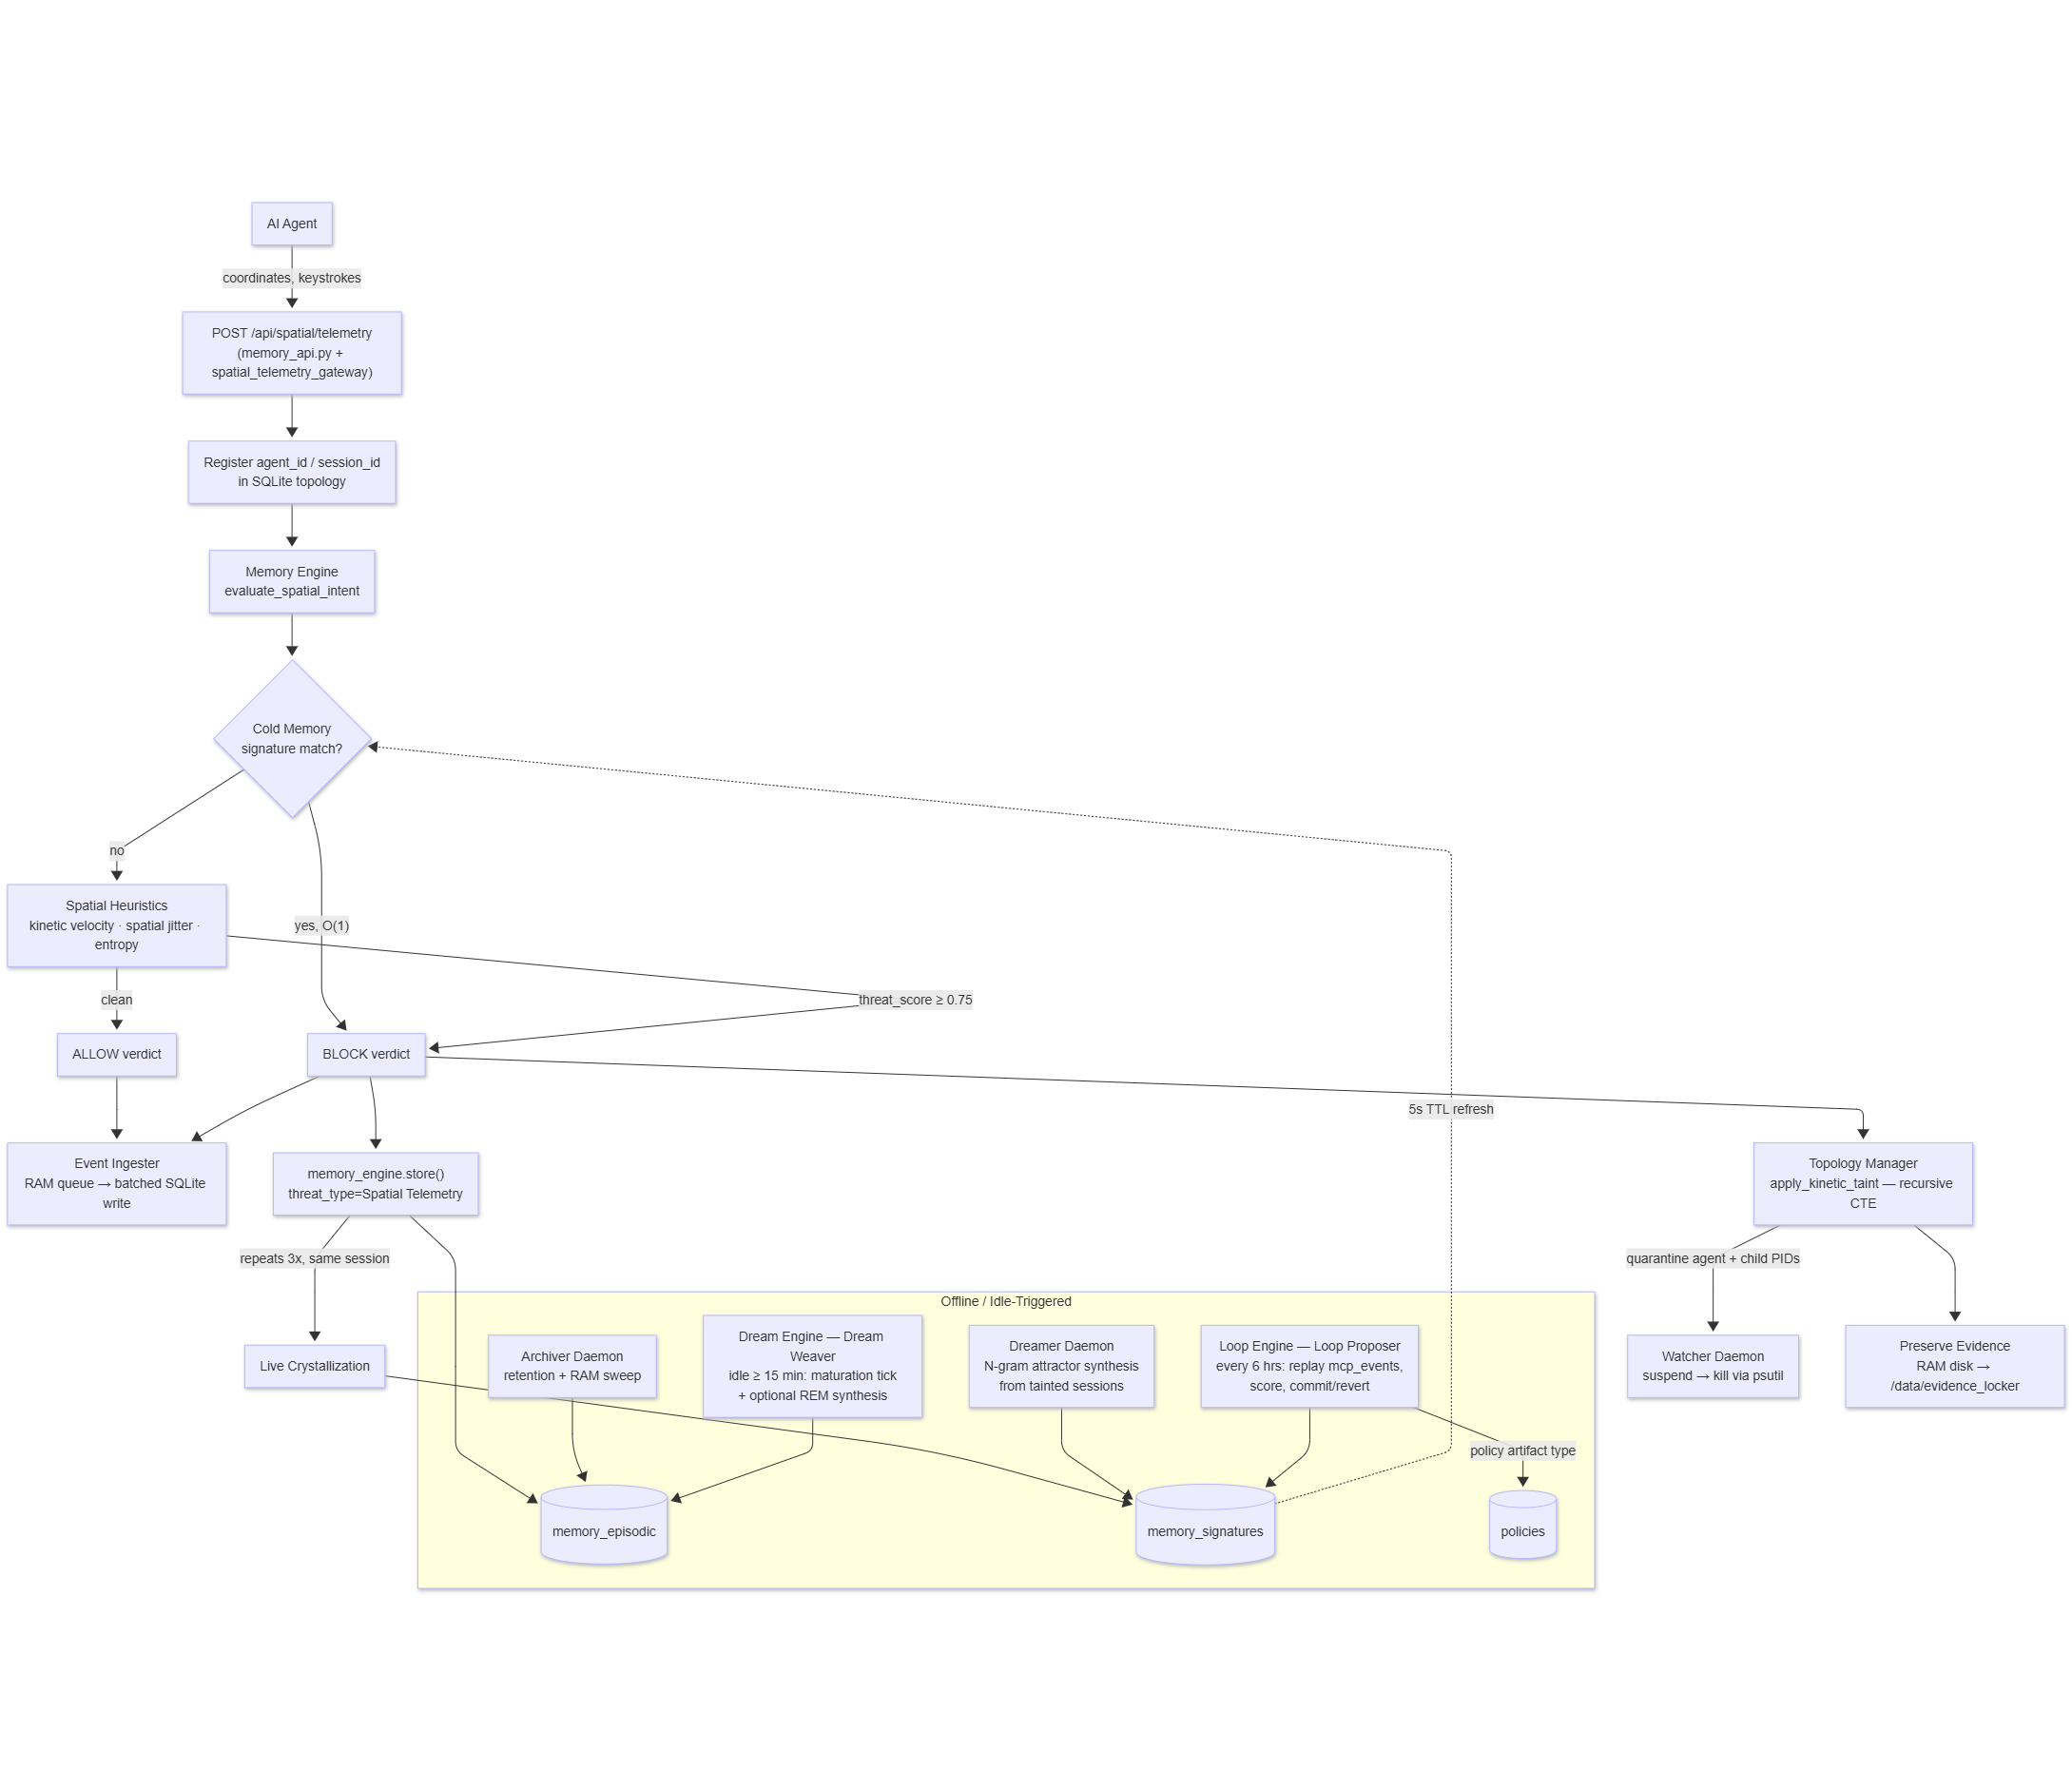
\includegraphics[width=\linewidth,height=0.85\textheight,keepaspectratio]{../diagrams/2.png}

\vspace{1.5em}

\caption{Spatial telemetry and memory data flow. Agent events enter the Memory Gateway, are
evaluated against Cold Memory signatures (fast path --- no LLM call), and routed through the
SpatialHeuristics engine. BLOCK verdicts are enforced directly by the Topology Manager and
Watcher Daemon, bypassing the signal loop entirely. ALLOW verdicts continue into the standard
pipeline.}
\label{fig:spatial}
\end{figure}

The memory substrate implements a three-tier architecture---\textsc{hot}, \textsc{warm}, and
\textsc{cold}---that mirrors the biological distinction between working memory, consolidating
recall, and crystallised long-term storage. It unifies two memory concerns that were developed in
parallel during v0.8.0: a \emph{deep} tier (episodic and semantic consolidation) and a
\emph{surface} tier (spatial telemetry and signature matching), merged into a single memory engine
so that telemetry flows through the same episodic/semantic lifecycle as every other verdict rather
than maintaining two disconnected substrates.

{\small
\begin{longtable}{L{1.6cm} L{3.6cm} L{5.0cm} L{4.0cm}}
\caption{The three-tier ButterClaw memory architecture.}\label{tab:memory-tiers}\\
\toprule
\textbf{Tier} & \textbf{Storage} & \textbf{Persistence / Transition} & \textbf{Primary Consumer} \\
\midrule
\endfirsthead
\multicolumn{4}{l}{\small\itshape Table~\thetable{} (continued)}\\
\toprule
\textbf{Tier} & \textbf{Storage} & \textbf{Persistence / Transition} & \textbf{Primary Consumer} \\
\midrule
\endhead
\midrule
\multicolumn{4}{r}{\small\itshape continued on next page}\\
\endfoot
\bottomrule
\endlastfoot
HOT & In-process working context (e.g.\ the five most recent successful tool-call events) & Held in RAM for the active session; no durable table of its own & Guardian Brain, Auditor (behavioral drift / \texttt{timeline\_context}) \\
WARM & \texttt{memory\_episodic} (SQLite) & Sigmoid \texttt{activation\_strength} maturation; records that sustain reinforcement are promoted into the \texttt{memory\_semantic} graph by the periodic maturation tick & Dream Weaver, Loop Proposer (pattern recall and consolidation) \\
COLD & \texttt{memory\_signatures} (SQLite) & Crystallises from the semantic graph after sustained repetition within a single session (an identical trajectory recurring 3+ times); provides an O(1) fast-path match; low-confidence entries decay over time & Fleet Sentinel, spatial heuristics fast path (signature matching with no LLM call) \\
\end{longtable}
}

\emph{Note on terminology:} the standalone \texttt{butterclaw-sentinel} SDK (\cref{sec:sdk})
exposes a simplified three-tier mirror of this substrate labelled HOT/EPISODIC/COLD for embedding
purposes; the two namings describe the same architectural concern at different levels of fidelity
and should not be conflated when citing tier behaviour.

The Dream Weaver and Loop Proposer hemispheres function as offline consolidation processes---they
do not participate in the real-time request pipeline and cannot issue BLOCK verdicts. The Dream
Weaver's cycle has two parts: unconditionally, a maturation tick that ages every episodic record's
activation strength, promotes matured entries into the semantic graph, prunes stale ones, and
decays low-confidence Cold Memory signatures; and, only when an LLM caller is configured, synthesis
of a speculative adversarial scenario from the most-observed semantic-graph entities, written back
with \texttt{source="dream"} and \texttt{verdict="SIMULATED"} so it can never be mistaken for a
live verdict. The Loop Proposer reads from COLD memory and the audit log, proposes one signature,
policy, or prompt change, replays it against recent \texttt{mcp\_events} through a side-effect-free
shadow evaluator, scores baseline against candidate, and commits or reverts---writing to a cold
store pending human review when operating in dry-run mode. Neither hemisphere can modify policy
files directly; the human-in-the-loop gate is architectural, not procedural, and the Loop
Proposer is explicitly barred from writing to \texttt{.py} targets at runtime.

Figure~\ref{fig:spatial} traces this pathway. A second, independent kinetic pathway runs beside
the Guardian-Brain-mediated one described above. Agent telemetry events are evaluated first
against the COLD Memory signature cache (an O(1)
fast path refreshed on a short interval, requiring no LLM call); only on a cache miss does a
slower heuristic evaluator score kinetic velocity, spatial jitter, and string entropy against the
most recent window of that session's telemetry. A \texttt{BLOCK} verdict from this fast path is
enforced directly---bypassing the Guardian Brain / DRIFT / Paranoia Dial chain entirely---which is
why its correctness depends so heavily on the same crystallisation discipline (3+ repeats
\emph{within one session}, never pooled across unrelated sessions) that governs ordinary Cold
Memory promotion.

\subsection{Fleet Detection Stack}
\label{sec:fleet}

Beginning in v0.9.0, ButterClaw extends single-agent containment with a fleet layer that reasons
about relationships \emph{between} agents rather than events within one agent's stream. Three
components implement this: a directed, weighted \textbf{Trust Graph} recording inter-agent
relationships and propagating taint along recorded edges; a \textbf{Collusion Detector} that
treats collusion roles---\texttt{encoder}, \texttt{exfiltrator}, \texttt{persister},
\texttt{scout}, \texttt{injector}---as properties of individual \emph{signature hit events} rather
than static agent attributes, matched against default complementary pairs
(\texttt{encoder}$\leftrightarrow$\texttt{exfiltrator}, \texttt{scout}$\leftrightarrow$
\texttt{injector}, \texttt{persister}$\leftrightarrow$\texttt{exfiltrator},
\texttt{encoder}$\leftrightarrow$\texttt{persister}, \texttt{scout}$\leftrightarrow$
\texttt{persister}); and the Fleet Sentinel hemisphere (\cref{sec:hemispheres}) that synthesises
both into a fleet-scope verdict.

Fleet state is deliberately isolated from single-agent state: the fleet database and the core
runtime database are never co-transacted, so a fault in fleet reasoning cannot corrupt
single-agent containment state, and vice versa. A low trust score alone never kills a process or
blocks a session directly---it informs the Fleet Sentinel only; kinetic action still flows through
the Guardian Brain, DRIFT, and the Paranoia Dial. This is the architecture's central fleet-layer
commitment: \emph{the Fleet Sentinel perceives; the existing exoskeleton decides.} Taint
propagation along the Trust Graph defaults to one hop and requires explicit configuration to
extend to two; it is never automated beyond that. Cross-fleet promotion of an entity from
session-scope to fleet-scope memory requires a human gate---no automated code path may perform
that promotion. The Threat Signature Arsenal remains the single signature system for both
individual-agent and collusion detection, so individual and fleet-level pattern matching can never
drift out of sync with one another.

\subsection{Comparison with Conventional Frameworks}

\begin{table}[htbp]
  \centering\small
  \caption{ButterClaw vs.\ Conventional Agentic Frameworks}
  \label{tab:comparison}
  \begin{tabularx}{\linewidth}{L{2.8cm} L{5.2cm} L{5cm}}
    \toprule
    \textbf{Dimension} & \textbf{Conventional Frameworks} & \textbf{ButterClaw} \\
    \midrule
    Isolation Model    & Shared context by default; isolation optional and app-managed & Isolation by default; sharing requires explicit policy authorization \\
    Loop Control       & Max iterations at app layer; not architecturally enforced & Hard depth limits at Layer~3; invariant violations trigger automated response \\
    Audit Surface      & Logging optional; replay not supported & Append-only chained audit log; full replay capability \\
    Kill Switch        & Process termination only; no state preservation; orphans common & Three-tier model with state preservation, drain, and orphan detection; concrete credential destruction (Gibson) \\
    Consent Mechanism  & Ad hoc per-application dialogs & Structured consent surfaces per signal class in policy graph; allow-never-short-circuits invariant (I-05) \\
    Multi-Agent Reasoning & Not architecturally distinguished from single-agent reasoning & Dedicated Fleet Sentinel hemisphere and Trust Graph, isolated from single-agent state \\
    \bottomrule
  \end{tabularx}
\end{table}

% ────────────────────────────────────────────────────────────────────────────
\section{Kill Switch Architecture}
\label{sec:killswitch}
% ────────────────────────────────────────────────────────────────────────────

\subsection{Why Kill Switches Fail}

Existing kill switch implementations fail in three systematic ways:

\textbf{Async Signal Orphaning}: Kill commands terminate the primary agent process but leave
asynchronously dispatched signals (to tool APIs, subagents, external services) executing in
flight. Those orphaned signals may complete, effect state changes, and spawn further signals
after the kill event.

\textbf{Context Persistence After Termination}: Context stored in shared caches or databases
survives process termination. A subsequent agent startup may inherit contaminated context,
effectively restarting the killed signal chain.

\textbf{Cascading Multi-Agent Signals}: Kill commands issued to one node in a multi-agent graph
do not automatically propagate to downstream agents that have already received derived signals.

\begin{warningbox}
A kill switch that terminates the process but does not resolve the signal graph is not a kill
switch. It is a process manager. The distinction is the difference between a system that stops
and one that continues mutating state under no active oversight.
\end{warningbox}

\subsection{The Three-Tier Kill Switch Model}

\textbf{Tier 1 --- Signal Pause}: Suspends all signal propagation. In-flight signals paused at
current routing hop; full state checkpointed. \emph{Reversible}. Appropriate for non-urgent
anomalies requiring human review.

\textbf{Tier 2 --- Loop Drain}: Blocks new initiations; allows in-flight signals to complete to
their nearest resolution checkpoint. Signals that do not resolve at that checkpoint are paused
and do not re-enter the routing loop. Appropriate for planned wind-downs or moderate anomalies.

\textbf{Tier 3 --- Hard Termination}: Immediately voids all active signals. State snapshot saved
to forensic store; forensic store locked. All signal identifiers written to orphan watchlist.
Subsequent callbacks matching those identifiers quarantined. Appropriate for confirmed harmful
behavior, security incidents, or regulatory directives. In the reference implementation, Tier~3
is the point at which the Gibson credential-destruction sequence (\cref{sec:gibson}) is triggered.

\subsection{Kill Switch Triggers}

\textbf{Manual}: Authorized human operator selects tier via operations interface.\\
\textbf{Automated}: Loop Monitor invariant violation exceeds severity threshold; tier determined
by severity configuration. In the reference implementation this is realised by the Paranoia Dial:
Level~2 terminates the offending process, and Level~3 triggers Gibson and system lockdown.\\
\textbf{Federated}: Peer agent or governance layer issues cryptographically attested cross-system
kill command; verified by receiving system's routing engine before execution.

\subsection{The Orphan Signal Problem}

Before any signal is dispatched to an external system, its identifier is registered in the orphan
watch registry. After a kill event, the registry is queried continuously; any callback, webhook,
or return signal matching a registered identifier is intercepted at Layer~0, classified as an
orphan, quarantined, logged, and presented to human review.

\subsection{Recovery and Re-Entry Protocols}

Re-entry after a kill event requires: (1)~resolution of all orphan activity; (2)~context membrane
flush and re-initialization; (3)~audit log review and root cause determination; (4)~routing
policy review and update for the signal class that caused the violation.

\begin{table}[htbp]
  \centering\small
  \caption{Kill Switch Tier Summary}
  \label{tab:killswitch}
  \begin{tabularx}{\linewidth}{L{2.2cm} L{3cm} L{3cm} L{2.5cm} L{3cm}}
    \toprule
    \textbf{Tier} & \textbf{Trigger} & \textbf{Signal Fate} & \textbf{State Fate} & \textbf{Recovery} \\
    \midrule
    1: Pause          & Non-urgent anomaly; human review needed      & Suspended at hop; state preserved    & Checkpoint written; memory retained   & Resume from checkpoint after clearance \\
    2: Loop Drain     & Planned wind-down; moderate anomaly          & Complete current cycle; no new init  & Resolved closed; unresolved paused    & Fresh init after quiesce \& policy review \\
    3: Hard Terminate & Confirmed harm; security incident; directive & Immediately voided; orphan watchlist & Forensic snapshot; store locked; credential vault destroyed (Gibson) & Full RCA; membrane flush; re-authorization \\
    \bottomrule
  \end{tabularx}
\end{table}

\subsection{Gibson: Concrete Credential Wipe Implementation}
\label{sec:gibson}

Where \cref{sec:killswitch} above describes the kill switch in the abstract, the reference
implementation's Tier~3 response includes a concrete, named mechanism---\textbf{Gibson}---for
destroying credential material so that a compromised or misbehaving deployment cannot continue to
authenticate after termination. Gibson is triggered by a Paranoia Level~3 verdict or by a manual
administrator call, and it executes as three atomic steps: (1)~every ciphertext row in the
credential vault is overwritten with cryptographic garbage, encrypted under a freshly generated,
immediately discarded Fernet ``poison'' key; (2)~every HMAC-SHA256 API key hash is deleted; and
(3)~the in-memory session-signing key cache is invalidated. If a hardcoded, non-configurable
\texttt{DRY\_RUN} flag is set, the sequence returns immediately without touching any of the three
---a pattern deliberately mirrored by the Dream Weaver's own non-overridable dry-run flag
(\cref{sec:memory}), because both guard against an irreversible action being taken by a process
that was never meant to take one.

Two design choices make Gibson something more than an undifferentiated wipe. First, because
session tokens are HMAC-signed with a key derived from the vault's master key, destroying the
vault automatically renders every active session cryptographically unverifiable---there is no
separate ``revoke all sessions'' step to forget. Second, and deliberately asymmetric: \emph{policy
rules and accumulated memory survive Gibson by design.} Wiping containment policy or learned
behavioral memory during incident response would leave the system defenseless at the moment of
re-authorization, so the credential wipe and the preservation of policy/memory are two expressions
of the same underlying principle---an incident should strip an attacker's standing access without
also stripping the defender's accumulated containment knowledge.

% ────────────────────────────────────────────────────────────────────────────
\section{The Signal Containment Model}
\label{sec:containment}
% ────────────────────────────────────────────────────────────────────────────

\subsection{Containment as a First-Class Design Primitive}

In ButterClaw, containment is defined \emph{before} the functional architecture. The routing 
engine, context membrane, loop monitor, and kill switch are not additions to the signal
processing system---they \emph{are} the signal processing system. Functionality is implemented
within the constraints they define, not despite them. This inversion is the central architectural
commitment of ButterClaw, and it is not achievable by retrofitting containment onto an existing
unconstrained agentic framework.

\subsection{The Four Containment Primitives}

\begin{definitionbox}[title=Definition 7.1 --- The Four Containment Primitives]
\textbf{Boundary}: A signal cannot cross defined perimeters without explicit authorization,
enforced jointly by the routing engine and context membrane.\

\vspace{4pt}
\textbf{Depth}: Recursion/loop depth is hard-bounded; signals at the limit route to an
escalation queue, not to further recursion.\

\vspace{4pt}
\textbf{Consent}: Any action modifying external state requires a verified consent authorization,
recorded in the provenance and audit log.\

\vspace{4pt}
\textbf{Observability}: Every signal event is logged to the append-only audit store in real time.
Audit store unavailability triggers system-wide Tier~1 kill; it is a precondition for operation.
\end{definitionbox}

\subsection{Formal Properties}

\begin{property}[Safety]
For every external state change $s$ effected by the system, there exists a consent authorization
record $c$ in the audit log that precedes $s$ and explicitly authorizes the action class of $s$.
\end{property}

\begin{property}[Liveness]
For every signal $\sigma$ with initiation time $t_0$, there exists a terminal event (resolution,
escalation, or kill) before $t_0 + T_{\max}$, where $T_{\max}$ is the configured maximum signal
lifetime.
\end{property}

\begin{property}[Fairness]
For every signal class $C$ and every time window $W$, signals of class $C$ that enter during $W$
receive routing attention proportional to their configured priority weight.
\end{property}

\subsection{Containment Threat Matrix}

\begin{table}[htbp]
  \centering\small
  \caption{Containment Threat Matrix}
  \label{tab:threats}
  \begin{tabularx}{\linewidth}{L{4.2cm} L{2.8cm} L{6cm}}
    \toprule
    \textbf{Threat} & \textbf{Primitive Violated} & \textbf{ButterClaw Mitigation} \\
    \midrule
    Signal crosses domain boundary without authorization  & Boundary          & Routing engine policy graph blocks; signal quarantined \& alert issued \\
    Recursive subagent spawning causes loop divergence    & Depth             & Hard depth limit; signal at limit routed to escalation queue; automated Tier~1 kill \\
    Signal modifies external state without human awareness & Consent          & Consent surface required; policy must explicitly authorize silent consent; audit preserved \\
    Signal executes without audit log entry               & Observability     & Audit store unavailability triggers system-wide Tier~1 kill \\
    Adversarial prompt injected into signal payload       & Boundary + Obs.   & Context membrane payload auth detects modification; Layer~0 adversarial classifier; quarantine \\
    Loop amplification attack                             & Depth + Obs.      & Signal initiation rate tracking; rapid initiation triggers Tier~2 kill; depth hard limit \\
    Context contamination across signal boundaries        & Boundary          & Context membrane enforces per-signal scoping; cross-signal sharing requires explicit auth event \\
    \bottomrule
  \end{tabularx}
\end{table}

\subsection{Implementation Mapping}
\label{sec:invariant-mapping}

The four containment primitives above are deliberately abstract so that they generalise beyond any
one implementation. Table~\ref{tab:invariant-mapping} maps them onto the specific, numbered
invariants enforced in the v0.9.2 reference implementation---the concrete claims an auditor could
check against the running system rather than against the architecture alone.

{\small
\begin{longtable}{L{2.2cm} L{2.6cm} L{10.3cm}}
\caption{Containment primitives mapped to enforced implementation invariants (v0.9.2).}\label{tab:invariant-mapping}\\
\toprule
\textbf{Primitive} & \textbf{Invariant(s)} & \textbf{Concrete Guarantee} \\
\midrule
\endfirsthead
\multicolumn{3}{l}{\small\itshape Table~\thetable{} (continued)}\\
\toprule
\textbf{Primitive} & \textbf{Invariant(s)} & \textbf{Concrete Guarantee} \\
\midrule
\endhead
\midrule
\multicolumn{3}{r}{\small\itshape continued on next page}\\
\endfoot
\bottomrule
\endlastfoot
Boundary & I-01, I-02, I-06, I-07-fleet & The vault master key exists only in the OS keyring and is never written to disk, env vars, or logs (I-01); all stored credentials pass through Fernet encryption before being written, so a compromised database file without the master key yields only ciphertext (I-02); only one watcher instance may run per host, enforced by a PID lock (I-06); the fleet database and the core runtime database are never co-transacted, so a fault in one cannot corrupt the other (I-07-fleet). \\
Depth & I-07, I-08, I-05-fleet & \texttt{ChainExecutor} enforces a hard ceiling of ten steps per chain under a sixty-second total timeout (I-07); the watcher retry queue is capped at 100 entries, with excess silently dropped rather than unbounded (I-08); cross-agent taint propagation defaults to one hop and requires explicit configuration, never automated, to extend to two (I-05-fleet). \\
Consent & I-05, I-02-fleet, I-04-fleet & An \textsc{allow} policy verdict is logged but never short-circuits evaluation of subsequent rules in the same scope (I-05, \cref{sec:drift}); a trust score of zero does not itself kill a process or block a session---it only informs the Fleet Sentinel, and kinetic action still requires the Guardian Brain + DRIFT + Paranoia Dial chain (I-02-fleet, I-04-fleet). \\
Observability & I-03, I-04, I-09, I-10 & The Gibson credential-wipe sequence executes as three explicitly ordered, auditable steps rather than an undifferentiated wipe (I-03, \cref{sec:gibson}); session-signing keys derive from the vault master key, so a wiped vault deterministically invalidates every session rather than leaving ambiguous state (I-04); the log sanitizer is a targeted blacklist, not an aggressive whitelist, preserving enough structure for the Guardian Brain to evaluate full prompt-injection attempts rather than silently discarding evidence of them (I-09); inbound transport reads are bounded at the byte level before the JSON parser engages, preventing an out-of-memory crash from silently destroying audit evidence (I-10). \\
\end{longtable}
}

% ────────────────────────────────────────────────────────────────────────────
\section{Related Work}
\label{sec:relatedwork}
% ────────────────────────────────────────────────────────────────────────────

\subsection{Agent Frameworks}

The conventional-frameworks comparison in Table~\ref{tab:comparison} is deliberately framed
against a generic baseline rather than any single project, because containment posture is uneven
across the ecosystem rather than uniformly absent. Composability-first frameworks such as
LangChain~\cite{chase2022langchain} and reasoning-and-acting formulations such as
ReAct~\cite{yao2023react} treat iteration limits, tool-call scoping, and audit logging as
application-layer concerns left to the integrator, not as architectural guarantees the framework
itself enforces. Multi-agent orchestration frameworks such as
AutoGen~\cite{wu2023autogen} and role-based software-engineering agent societies such as
MetaGPT~\cite{hong2023metagpt} extend this same pattern to inter-agent communication: they
standardise \emph{how} agents exchange messages and delegate subtasks, but leave isolation,
consent, and kill-switch semantics to the surrounding deployment. Generative-agent simulations of
believable human behavior~\cite{park2023generative} and self-reflective agents that revise their
own trajectories based on verbal feedback~\cite{shinn2023reflexion} further illustrate the trend
this paper argues against: capability and autonomy have grown fastest in exactly the dimensions
(memory, self-revision, multi-agent delegation) that the signal model frame identifies as the new
safety surface, without a corresponding growth in architecturally-enforced containment.

\subsection{Prompt Injection}

The context membrane (\cref{sec:butterclaw}) and the DRIFT policy engine's payload scanning
(\cref{sec:drift}) are ButterClaw's responses to a threat class documented extensively in prior
work. Indirect prompt injection via untrusted retrieved content was characterised
by~\cite{greshake2023injection} as a structural consequence of LLM applications that cannot
distinguish instructions from data at the point of ingestion; earlier adversarial prompting
work~\cite{perez2022ignore} and the broader survey of injection attacks and
defenses~\cite{liu2023promptinjection} establish that filtering at the output stage---the
conventional ``language model'' response---does not address injection that occurs upstream, at
the point where untrusted content enters the context window. This paper's signal model framing
reframes the same threat as a \emph{boundary} violation (Definition~7.1) enforced at ingestion
(Layer~1) rather than a content-moderation problem addressed after the fact.

\subsection{Kill Switch Research}

The theoretical foundation for corrigibility and safe interruptibility predates this paper's
architecture by nearly a decade. The off-switch game~\cite{hadfieldmenell2017offswitch} formalises
the incentive problem---an agent optimising a fixed objective has no inherent reason to tolerate
being switched off, and corrigibility must be designed in rather than assumed. Safely
interruptible agents~\cite{orseau2016interruptible} and the technical research agenda for aligning
superintelligence~\cite{soares2014aligning} likewise treat interruptibility as a property that
must survive the agent's own learning process, not merely a process-management feature bolted on
afterward. ButterClaw's three-tier kill switch model and its orphan-signal watch registry
(\cref{sec:killswitch}) are an attempt to answer, at the systems-engineering level, the same
question this literature poses at the theoretical level: what does it mean for a termination
signal to actually terminate, rather than merely appearing to?

% ────────────────────────────────────────────────────────────────────────────
\section{Software Artifact and Reproducibility}
\label{sec:artifact}
% ────────────────────────────────────────────────────────────────────────────

\subsection{Repository}

The ButterClaw runtime described in this paper is released as open-source software under the
Apache-2.0 license at \url{https://github.com/butterclaw-tech/butterclaw}. The release
accompanying this whitepaper revision corresponds to runtime version \textbf{v0.9.2}, which
introduced the Fleet Detection Stack (\cref{sec:fleet}) and the fifth reasoning hemisphere on top
of the v0.8.0 memory and offline-consolidation substrate (\cref{sec:memory}).

\subsection{The butterclaw-sentinel SDK}
\label{sec:sdk}

Alongside the full runtime, a dependency-free, embeddable Python library---
\texttt{butterclaw-sentinel}---is released at
\url{https://github.com/butterclaw-tech/butterclaw-sdk}. The SDK ports seven internal subsystems
directly from the v0.9.2 source behind a single \texttt{Sentinel} facade: \texttt{SentinelCore}
(the three background daemons---fallback ticker, dream loop, loop engine), \texttt{AgentRegistry},
\texttt{PolicyEngine} (the DRIFT evaluator of \cref{sec:drift}), \texttt{TrustGraph},
\texttt{DriftDetector} (a generalisation of the spatial-telemetry heuristics of
\cref{sec:memory} to arbitrary numeric metrics, hardcoded to the v0.9.2 thresholds
\texttt{MAX\_TYPING\_VELOCITY=15.0} and a spatial-jitter threshold of 800), \texttt{CollusionDetector},
and \texttt{MemorySubstrate} (the SDK's HOT/EPISODIC/COLD mirror of the runtime's HOT/WARM/COLD
architecture; see the note in \cref{sec:memory}). The SDK exists to let integrators embed
ButterClaw's containment primitives---particularly the DRIFT evaluator and its I-05 invariant---
into a host application without running the full Flask server, and it carries the same core
invariants (I-13, I-14, I-15) forward into its own design-invariant register.

\subsection{Citation}

Researchers and practitioners building on this work should cite both the whitepaper (via its
Zenodo DOI, minted for this record) and, where the runtime itself is used, the software
repository directly:

\begin{lstlisting}[caption={Suggested citation form}]
Bc77. "Autonomous Signals: A New Ontology for AI Agents."
ButterClaw Tech, 2026. Zenodo. <DOI to be inserted on publication>.
Software: https://github.com/butterclaw-tech/butterclaw (v0.9.2)
SDK:      https://github.com/butterclaw-tech/butterclaw-sdk
\end{lstlisting}

\subsection{Version Binding}

This revision of the whitepaper is bound to runtime version \textbf{v0.9.2}. Readers should note
that the Zenodo record's own version field tracks the \emph{whitepaper's} revision history
(currently \texttt{v1.0.0} at time of writing) independently of the \emph{software's} semantic
version---the two are related but distinct, and a later whitepaper revision describing a later
runtime version will increment the Zenodo version without implying a corresponding software
major-version bump, or vice versa. Claims in Sections~\ref{sec:butterclaw}--\ref{sec:containment}
that cite specific temperatures, invariant IDs, or table/column names should be understood as
accurate as of v0.9.2 and re-verified against \href{https://github.com/butterclaw-tech/butterclaw/blob/main/docs/ARCHITECTURE.md}{\texttt{ARCHITECTURE.md}} before being relied upon
for a different runtime version.

\subsection{Practical Deployment}

The audit store's availability-as-prerequisite constraint demands that enterprises treat audit
infrastructure with the same reliability requirements as their primary data tier. Consent surface
design requires organizational policy work before technical implementation: which action classes
require interactive human consent, which are eligible for policy pre-authorization, and which
are never authorized regardless of instruction. This is a governance exercise, not an engineering
one.

\subsection{Interoperability}

ButterClaw wraps existing LLM APIs rather than replacing them. Model inference calls are signal
transformations executed within Layer~2; the API call is not modified. Existing agent frameworks
can be adapted by implementing adapters that translate framework-native constructs into
ButterClaw signal events before execution---the SDK's own three-method adapter contract
(\texttt{connect}/\texttt{adapt}/\texttt{sync}, \cref{sec:sdk}) is one concrete instance of this
pattern. Frameworks with opaque execution loops require deeper instrumentation or replacement with
ButterClaw-native components.

% ────────────────────────────────────────────────────────────────────────────
\section{Open Problems}
\label{sec:openproblems}
% ────────────────────────────────────────────────────────────────────────────

\textbf{Formal Verification of Loop Convergence}: Can convergence guarantees be provided for
signal loops containing learned model components? Recent work in neural network verification and
abstract interpretation provides partial tools, but the compositional complexity of multi-step
agentic loops with non-deterministic routing remains an open formal methods problem.

\textbf{Cross-Organizational Federated Kill Switches}: Kill switch coordination across
organizational boundaries becomes a multi-party protocol design problem. What consensus mechanism
governs cross-org kill events? What liability framework governs actions taken on the basis of a
federated kill signal? These are simultaneously technical, legal, and governance questions.

\textbf{Signal-Level Interpretability}: Current interpretability research focuses on individual
model inference internals. Signal-level interpretability asks why the system routed a signal a
particular way, and what accumulated context at each hop reveals about effective system
objectives---requiring new tools operating at the signal graph level.

\textbf{Automatic Containment Policy Generation}: Future work should explore whether containment
policies can be learned from operator demonstrations, with depth limits inferred from task
complexity distributions and consent surfaces adapted dynamically from signal behavior patterns.

% ────────────────────────────────────────────────────────────────────────────
\section{Conclusion}
\label{sec:conclusion}
% ────────────────────────────────────────────────────────────────────────────

This paper has argued for a fundamental ontological shift: from the language model frame---in
which the system is a text predictor and safety is a content property---to the signal model
frame, in which the system is a signal transducer and safety is an architectural property defined
at signal boundaries, depths, consent surfaces, and observability.

\begin{pullquotebox}
``We cannot engineer defenses against failure modes we cannot name. The signal model frame makes
the safety surface of autonomous AI systems legible for the first time.''
\end{pullquotebox}

ButterClaw is our proposal for what containment-first architecture looks like when signal model
thinking is taken seriously. Its six layers, five reasoning hemispheres, named DRIFT policy
engine, three-tier memory substrate, fleet detection stack, three kill switch tiers (with a
concrete credential-destruction mechanism), four containment primitives, and formal properties are
offered as a concrete engineering target---one we have mapped, invariant by invariant, onto a
running v0.9.2 implementation rather than leaving as architecture diagrams alone. We expect and
welcome disagreement about specific design choices. What we ask is that disagreement be conducted
at the signal level, not the token level.

The research and engineering community has built extraordinary systems. The next task is to
contain them---not to diminish their capability, but to ensure that capability is exercised
within boundaries that are legible, auditable, and subject to human control.

% ────────────────────────────────────────────────────────────────────────────
\bibliographystyle{unsrt}
% ────────────────────────────────────────────────────────────────────────────
\begin{thebibliography}{26}

\bibitem{amodei2016concrete}
D.~Amodei, C.~Olah, J.~Steinhardt, P.~Christiano, J.~Schulman, and D.~Man\'e.
\newblock Concrete problems in {AI} safety.
\newblock \textit{arXiv:1606.06565}, 2016.

\bibitem{anthropic2024spec}
Anthropic.
\newblock Claude's model specification.
\newblock \textit{Anthropic Technical Documentation}, 2024.

\bibitem{bai2022rlhf}
Y.~Bai, A.~Jones, K.~Ndousse, et~al.
\newblock Training a helpful and harmless assistant with reinforcement learning from human feedback.
\newblock \textit{arXiv:2204.05862}, 2022.

\bibitem{bommasani2021foundation}
R.~Bommasani, D.~A. Hudson, E.~Adeli, et~al.
\newblock On the opportunities and risks of foundation models.
\newblock \textit{Stanford CRFM Technical Report}, 2021.

\bibitem{brundage2018malicious}
M.~Brundage, S.~Avin, J.~Clark, et~al.
\newblock The malicious use of artificial intelligence: Forecasting, prevention, and mitigation.
\newblock \textit{Future of Humanity Institute Technical Report}, 2018.

\bibitem{chase2022langchain}
H.~Chase.
\newblock {LangChain}: Building applications with {LLM}s through composability, 2022--2024.
\newblock \url{https://github.com/langchain-ai/langchain}. Accessed October 2026; repository has
  no single pinned release corresponding to the framework behavior discussed here.

\bibitem{christiano2017rlhf}
P.~Christiano, J.~Leike, T.~Brown, et~al.
\newblock Deep reinforcement learning from human preferences.
\newblock In \textit{NeurIPS 2017}.

\bibitem{greshake2023injection}
K.~Greshake, S.~Abdelnabi, S.~Mishra, C.~Endres, T.~Holz, and M.~Fritz.
\newblock Not what you've signed up for: Compromising real-world {LLM}-integrated applications
  with indirect prompt injection.
\newblock In \textit{Proceedings of the 16th ACM Workshop on Artificial Intelligence and Security
  (AISec)}, 2023.

\bibitem{hadfield2017inverse}
D.~Hadfield-Menell, S.~Milli, P.~Abbeel, S.~Russell, and A.~Dragan.
\newblock Inverse reward design.
\newblock In \textit{NeurIPS 2017}.

\bibitem{hadfieldmenell2017offswitch}
D.~Hadfield-Menell, A.~Dragan, P.~Abbeel, and S.~Russell.
\newblock The off-switch game.
\newblock In \textit{Proceedings of the 26th International Joint Conference on Artificial
  Intelligence (IJCAI)}, 2017.

\bibitem{hong2023metagpt}
S.~Hong, X.~Zheng, J.~Chen, et~al.
\newblock {MetaGPT}: Meta programming for a multi-agent collaborative framework.
\newblock \textit{arXiv:2308.00352}, 2023.

\bibitem{leike2017gridworlds}
J.~Leike, M.~Martic, V.~Krakovna, et~al.
\newblock {AI} safety gridworlds.
\newblock \textit{arXiv:1711.09883}, 2017.

\bibitem{liu2023promptinjection}
Y.~Liu, G.~Deng, Y.~Li, et~al.
\newblock Prompt injection attacks and defenses in {LLM}-integrated applications.
\newblock \textit{arXiv:2310.12815}, 2023.

\bibitem{minsky1986society}
M.~Minsky.
\newblock \textit{The Society of Mind}.
\newblock Simon and Schuster, 1986.

\bibitem{openai2023gpt4}
OpenAI.
\newblock {GPT-4} technical report.
\newblock \textit{arXiv:2303.08774}, 2023.

\bibitem{orseau2016interruptible}
L.~Orseau and S.~Armstrong.
\newblock Safely interruptible agents.
\newblock In \textit{Proceedings of the 32nd Conference on Uncertainty in Artificial Intelligence
  (UAI)}, 2016.

\bibitem{park2023generative}
J.~S. Park, J.~C. O'Brien, C.~J. Cai, et~al.
\newblock Generative agents: Interactive simulacra of human behavior.
\newblock In \textit{ACM UIST 2023}.

\bibitem{perez2022ignore}
F.~Perez and I.~Ribeiro.
\newblock Ignore previous prompt: Attack techniques for language models.
\newblock \textit{arXiv:2211.09527}, 2022.

\bibitem{russell2019human}
S.~Russell.
\newblock \textit{Human Compatible: Artificial Intelligence and the Problem of Control}.
\newblock Viking Press, 2019.

\bibitem{shavit2023chinchilla}
Y.~Shavit.
\newblock What does it take to catch a chinchilla? verifying rules on large-scale neural network training runs.
\newblock \textit{arXiv:2303.11341}, 2023.

\bibitem{shinn2023reflexion}
N.~Shinn, F.~Cassano, A.~Gopinath, K.~Narasimhan, and S.~Yao.
\newblock Reflexion: Language agents with verbal reinforcement learning.
\newblock In \textit{NeurIPS 2023}.

\bibitem{soares2014aligning}
N.~Soares and B.~Fallenstein.
\newblock Aligning superintelligence with human interests: A technical research agenda.
\newblock \textit{MIRI Technical Report 2014-8}, 2014.

\bibitem{weng2023llmagents}
L.~Weng.
\newblock {LLM}-powered autonomous agents.
\newblock \textit{Lilian Weng's Blog, OpenAI}, 2023.
\newblock \url{https://lilianweng.github.io/posts/2023-06-23-agent/}.

\bibitem{wu2023autogen}
Q.~Wu, G.~Bansal, J.~Zhang, et~al.
\newblock {AutoGen}: Enabling next-gen {LLM} applications via multi-agent conversation.
\newblock \textit{arXiv:2308.08155}, 2023.

\bibitem{yao2023react}
S.~Yao, J.~Zhao, D.~Yu, et~al.
\newblock {ReAct}: Synergizing reasoning and acting in language models.
\newblock In \textit{ICLR 2023}.

\bibitem{ziegler2019finetuning}
D.~M. Ziegler, N.~Stiennon, J.~Wu, et~al.
\newblock Fine-tuning language models from human preferences.
\newblock \textit{arXiv:1909.08593}, 2019.

\end{thebibliography}

\end{document}
